% --- Template for thesis / report with tktltiki2 class ---
% 
% last updated 2013/02/15 for tkltiki2 v1.02

\documentclass[finnish]{tktltiki2}

% tktltiki2 automatically loads babel, so you can simply
% give the language parameter (e.g. finnish, swedish, english, british) as
% a parameter for the class: \documentclass[finnish]{tktltiki2}.
% The information on title and abstract is generated automatically depending on
% the language, see below if you need to change any of these manually.
% 
% Class options:
% - grading                 -- Print labels for grading information on the front page.
% - disablelastpagecounter  -- Disables the automatic generation of page number information
%                              in the abstract. See also \numberofpagesinformation{} command below.
%
% The class also respects the following options of article class:
%   10pt, 11pt, 12pt, final, draft, oneside, twoside,
%   openright, openany, onecolumn, twocolumn, leqno, fleqn
%
% The default font size is 11pt. The paper size used is A4, other sizes are not supported.
%
% rubber: module pdftex

% --- General packages ---

\usepackage[utf8]{inputenc}
\usepackage[T1]{fontenc}
\usepackage{lmodern}
\usepackage{microtype}
\usepackage{amsfonts,amsmath,amssymb,amsthm,booktabs,color,enumitem,graphicx}
\usepackage[pdftex,hidelinks]{hyperref}
\usepackage{listings}
\usepackage{xcolor}
\usepackage{amsmath}
\usepackage{graphicx}
\usepackage{sidecap}
\usepackage{setspace}
\onehalfspacing
\lstset{
	keywordstyle=\color{black}\bfseries, % style for keywords
	numbers=none, % where to put the line-numbers
	numberstyle=\tiny, % the size of the fonts that are used for the line-numbers     
	showspaces=false, % shcow spaces adding particular underscores
	showstringspaces=false, % underline spaces within strings
	showtabs=false, % show tabs within strings adding particular underscores
	frame=single, % adds a frame around the code
	framesep=5pt,
	aboveskip=15pt,
	belowskip=15pt,
	tabsize=2, % sets default tabsize to 2 spaces
	rulesepcolor=\color{gray},
	rulecolor=\color{black},
	captionpos=b, % sets the caption-position to bottom
	breaklines=true, % sets automatic line breaking
	breakatwhitespace=false,
	literate={ö}{{\"o}}1
	{ä}{{\"a}}1
	{ü}{{\"u}}1
}

% Automatically set the PDF metadata fields
\makeatletter
\AtBeginDocument{\hypersetup{pdftitle = {\@title}, pdfauthor = {\@author}}}
\makeatother

% --- Language-related settings ---
%
% these should be modified according to your language

% babelbib for non-english bibliography using bibtex
\usepackage[fixlanguage]{babelbib}
\selectbiblanguage{finnish}

% add bibliography to the table of contents
\usepackage[nottoc]{tocbibind}
% tocbibind renames the bibliography, use the following to change it back
\settocbibname{Lähteet}

% --- Theorem environment definitions ---

\newtheorem{lau}{Lause}
\newtheorem{lem}[lau]{Lemma}
\newtheorem{kor}[lau]{Korollaari}

\theoremstyle{definition}
\newtheorem{maar}[lau]{Määritelmä}
\newtheorem{ong}{Ongelma}
\newtheorem{alg}[lau]{Algoritmi}
\newtheorem{esim}[lau]{Esimerkki}

\theoremstyle{remark}
\newtheorem*{huom}{Huomautus}


% --- tktltiki2 options ---
%
% The following commands define the information used to generate title and
% abstract pages. The following entries should be always specified:

\title{SQL-Injektio ja siltä suojautuminen}
\author{Lalli Nuorteva}
\date{\today}
\level{Kandidaatintutkielma}
\abstract{Tämän kandidaatintutkielman päätavoite on selvittää mitä keinoja SQL-injektiolta suojautumiseen on olemassa. Tutkielma koostuu seuraavista osa-alueista: SQL-injektion esittely, tietoturvallisen ohjelman toteutus, ajonaikainen SQL-injektioiden estäminen ja penetraatiotestaus. 

Menetelmiin perehdytään siten, että lukija ymmärtää kuinka ne toimivat. Kun ohjelmoija ymmärtää miten hänen valmitsemansa suojautumismetodit toimivat, hän tuntee myös suojauksen heikkoudet ja vahvuudet.}

% The following can be used to specify keywords and classification of the paper:

\keywords{SQL-injektio}

% classification according to ACM Computing Classification System (http://www.acm.org/about/class/)
% This is probably mostly relevant for computer scientists
% uncomment the following; contents of \classification will be printed under the abstract with a title
% "ACM Computing Classification System (CCS):"
% \classification{}

% If the automatic page number counting is not working as desired in your case,
% uncomment the following to manually set the number of pages displayed in the abstract page:
%
% \numberofpagesinformation{16 sivua + 10 sivua liitteissä}
%
% If you are not a computer scientist, you will want to uncomment the following by hand and specify
% your department, faculty and subject by hand:
%
% \faculty{Matemaattis-luonnontieteellinen}
% \department{Tietojenkäsittelytieteen laitos}
% \subject{Tietojenkäsittelytiede}
%
% If you are not from the University of Helsinki, then you will most likely want to set these also:
%
% \university{Helsingin Yliopisto}
% \universitylong{HELSINGIN YLIOPISTO --- HELSINGFORS UNIVERSITET --- UNIVERSITY OF HELSINKI} % displayed on the top of the abstract page
% \city{Helsinki}
%


\begin{document}
	
	% --- Front matter ---
	\frontmatter      % roman page numbering for front matter
	
	\maketitle        % title page
	%\makeabstract     % abstract page
	
	\makeabstract
	
	\tableofcontents  % table of contents
	
	% --- Main matter ---
	
	\mainmatter       % clear page, start arabic page numbering
	
	\section{Johdanto}
	Viime aikoina entistä useampi palvelu on siirtynyt verkkoon. Tämän seurauksena verkossa käsitellään jatkuvasti entistä enemmän arkaluonteisia tietoja. Verkossa hoidetaan asioita kuten laskujen maksaminen, hotellien varaus ja henkilökohtaisten viestien vaihtaminen. Yleensä tiedot tallennetaan relaatiotietokantoihin. Juuri tällaiset sovellukset voivat olla haavoittuvaisia SQL-injektioille, ellei niiltä olla suojauduttu oikeaoppisesti. Tästä syystä jokaisen tietokantasovelluksia ohjelmoivan on ymmärrettävä mikä on SQL-injektio ja kuinka siltä voidaan suojautua.
	
	Tutkimusten mukaan kahdeksan prosenttia web-palveluista sisältää haavoittuvuuksia.  87 Prosenttia näistä haavoittuvuuksista on SQL-injektio haavoittuvuuksia \cite{detection}. Yleisyytensä lisäksi SQL-injektio on myös hyvin vaarallinen. Onnistuneen SQL-injektion avulla hyökkääjä voi suorittaa huonosti suojatussa tietokannassa mitä tahansa operaatioita. Tämä voi mahdollistaa esimerkiksi arkaluontoisten tietojen lukemisen ja muokkaamisen, tai esimerkiksi sovelluksen autentikaation ohittamisen. SQL-Injektio mielletään monesti amatöörien ongelmaksi, mutta sen avulla on murrettu myös paljon ammattilaisten toteuttamia järjestelmiä. Yksi suurimmista SQL-injektion avulla tehdyistä murroista tehtiin Guess.com:ille \cite{guess}. Hyökkääjä sai tietoonsa 200 000 ihmisen nimet ja luottokorttitiedot.
	
	Sen lisäksi että SQL-injektio on yleisin tietoturva-aukko, se on myös helppoa toteuttaa ilman syvällistä ymmärrystä sen toiminnasta. Esimerkiksi penetraatiotestaustyökalut , kuten "sqlmap"\space, ilmoittavat sivuston heikkouksista melkeinpä napin painalluksella. Vaikka sqlmapin kaltaiset työkalut onkin tehty nimenomaan penetraatiotestaukseen, mikään ei estä hyökkääjää käyttämästä niitä apunaan. Niinpä on tärkeää, että ohjelmoija tuntee yleisimmät penetraatiotestaustyökalut, sekä käyttää niitä.
	
	Toisaalta SQL-injektota ei ole vaikeaa estää, mikäli ohjelmoija ymmärtää kuinka SQL-injektio toimii. Nykyaikaiset web-applikaatioiden viitekehykset, sekä ohjelmointikielet tarjoavat työkaluja SQL-injektioiden torjumiseen. Työkalujen käytöstä on tehty niin yksinkertaista, että ohjelmoijan tarvitsee vain muistaa käyttää niitä oikeissa paikoissa lähdekoodia. Esimerkiksi Ruby on Rails:issa  "Model.find\_by\_something(parametri)"\space hoitaa itsestään parametrin tarkastamisen ja käsittelyn SQL-injektion varalta. SQL-Injektion estämisestä on tehty jopa niin helppoa, että jotkut saattavat erehtyä luulemaan, ettei ohjelmoijan tarvitse enää huolehtia siitä. Kuitenkin esimerkiksi Railsin "Model.where(parametri)"\space -metodi on altis SQL-injektoille. Niinpä ohjelmoija ei voi luottaa viitekehyksen tai ohjelmointikielen hoitavan automaattisesti kaikkea. Tästä syystä ymmärrys SQL-injektioiden toiminnasta on yhä nykyaikanakin välttämätöntä.  
	
	
	\section{SQL-Injektio}
	Anleyn artikkelin "Advancen SQL Injections in SQL Server Applications"\space\cite{definition}\space mukaan SQL-injektio hyökkäys esiintyy silloin, kun hyökkääjä pääsee muuttamaan SQL käskyn logiikkaa, semantiikkaa tai syntaksia. Tämä tapahtuu lisäämällä alkuperäiseen kyselyyn uusia SQL-avainsanoja tai operaattoreita.
	Mikäli sovelluksen tietokantaoikeuksia ei ole erikseen rajattu, hyökkääjä voi onnistuneen SQL-injektion seurauksena suorittaa mitä tahansa tietokantapalvelimen tukemia SQL-kyselyitä. Jotkut tietokantapalvelimet sallivat myös käyttöjärjestelmätason komentojen suorittamisen. Tällöin hyökkääjän on mahdollista suorittaa myös muunlaisia hyökkäyksiä. 
	
	SQL-Injektio on mahdollinen vain silloin kun käyttäjältä tulevaa tietoa käytetään osana tietokantapalvelimelle tehtävää kyselyä. Tämä on kuitenkin varsin tavallinen tarve sovelluksissa. Tietokannassa voidaan säilyttää esimerkiksi käyttäjätunnuksia ja salasanoja. Näin ollen kirjautuessa järjestelmään käyttäjän antamaa syötettä käytetään osana SQL-kyselyä.
	
	\subsection{SQL-Injektio käytännössä}
	
 Esimerkiksi tuotteiden etsimiseen liittyvä SQL-kysely voidaan toteuttaa SQL-injektiolle alttiissa sovelluksessa seuraavalla tavalla:
 
	\begin{lstlisting}
	sql = "SELECT * FROM tuotteet
	WHERE nimi ="'" + params[:tuotenimi] + "'"
	\end{lstlisting}
	
	Mikäli käyttäjä antaa nimekseen "\space'; DROP TABLE tuotteet'. Valmis kysely tietokannalle näyttää seuraavalta:
	
	\begin{lstlisting}[language=sql]
	sql = "SELECT * FROM tuotteet
	WHERE nimi =''; DROP TABLE tuotteet     
	\end{lstlisting}
	
	Kyseinen kysely etsii ensin kaikki tuotteet joiden nimi on tyhjä. Seuraavaksi suoritetaan komento "DROP TABLE tuotteet", joka poistaa koko tuotteet taulun.
	
	 Edellä mainitun hyökkäyksen sijaan hyökkääjä olisi voinut käyttää esimerkiksi jotakin Srivastavan artikkelissa "Algorithm to prevent back end database against SQL injection attacks"\space \cite{piggy} esitellyistä menetelmistä:  
		\begin{description}
			
		\item[Tautologia] \hfill
		
		Hyökkääjä voi käyttää tuotenimeä, joka sisältää jonkin tautologian esimerkiksi "'; OR 1=1". Tällöin hyökkääjä olisi saanut vastauksena kaikki tuotteet.
		
		\item[Kommentti] \hfill
		
		Mikäli tuote olisi vaatinut myös tuotekoodin, eli kyselyn muotoilu olisi ollut esimerkiksi seuraavanlainen:
			\begin{lstlisting}[language=sql]
				sql = "SELECT * FROM tuotteet
				WHERE nimi ='" + params[:tuotenimi] AND tuotekoodi ='"params[:tuotekoodi]"'
			\end{lstlisting}
			Hyökkääjä voi kirjoittaa tuotenimeksi "Haluttu tuote'; --". Hyökkäyksen onnistuessa loput kyselystä muuttuu kommentoiduksi. Tällöin tuotteen tiedot palautetaan, vaikka hyökkääjä ei tietäisi tuotekoodia. Kaksi viivaa on kommenttimerkki esimerkiksi Transact-SQL:llässä ja Micorosft SQL serverissä \cite{sqlids}.
			
		\item[Union kysely] \hfill
		
		Hyökkääjä voi kirjoittaa tuotenimeksi esimerkiksi "Haluttu tuote' UNION SELECT * FROM kayttajatiedot". Hyökkäyksen onnistuessa vastaukseen sisältyy myös koko taulun "kayttajatiedot"\space sisältö.
	\end{description}
	
	\subsection{Obfuskointi}
	
	Edellisen kappaleen esimerkit eivät todennäköisesti toimi sovelluksissa, jotka on suojattu SQL-injektioilta. Tästä syystä hyökkääjien on käytettävä tapoja, joilla palomuureja voidaan kiertää. Salgadon kirjoittaman "SQL Injection Optimization and Obfuscation Techniques"\space\cite{encoding} artikkelissa esitellään obfuskointia. Obfuskointi tarkoittaa koodin tahallista monimutkaistamista ja epäselkeyttämistä sen varsinaisen toiminnan piilottamiseksi. Obfuskointia käytetään esimerkiksi haittaohjelmien piilottamiseen virustutkilta. SQL-Injektoiden tapauksessa obfuskointi voi olla yksinkertaisimillaan esimerkiksi "DROP"\space avainsanan muuttaminen "DroP":iksi. Tällöin yksinkertainen mustalistaukseen perustuva palomuuri saattaisi päästää SQL-injektion läpi.
	
	Hienostuneemmat tavat saattavat käyttävät SQL-injektioiden piilottamiseen esimerkiksi erilaisia enkoodauksia. Salgagon mukaan enkoodauksien käyttö perustuu siihen, että eri kerrokset käsittelevät enkoodauksia eri tavalla. Esimerkiksi Unicodessa merkkiä "a"\space vastaa merkkijono "\%u0061".\space Voi olla että palomuuri tulkitsee merkkijonon "\%u0061"\space tavallisena merkkijonona, kun taas tietokanta tulkitsee sen kirjaimena "a". Näin ollen esimerkiksi avainsana SELECT voidaan piilottaa unicoden avulla merkkijonoon "\%u0053\%u0045\%u004c\%u0045\%u0043\%u0054".
	
	\subsection{SQL-Injektioiden luokittelu}
		Sadeghiani ja hänen kollegoidensa artikkelin "SQL-Injection is still alive"\space mukaan SQL-injektioita luokitellaan sen perusteella, miten
		 hyökkääjä saa palautteen sovellukselta. SQL-Injektioita on kolmea eri päätyyppiä, inband injektio, out-of-band injektio ja sokea injektio \cite{still-alive}.
	
	\subsubsection{Inband injektio}
	Artikkelin mukaan inband tyyppinen injektio on kyseessä silloin, kun vastaus saadaan samaa reittiä, jota hyökkäys on suoritettu. Tällainen aukko saattaa esiintyä esimerkiksi sovelluksessa, jossa hyökkääjä voi hakea ystäviensä lisäämiä kuvia. Hyökkäyksen tuloksena hyökkääjä voi saada esimerkiksi kaikki tietokannasta löytyvät kuvat.
	
	\subsubsection{Out-of-band injektio}
	Sen sijaan out-of-band injektiossa tuloste saadaan eri reittiä, kun hyökkäys on syötetty. Out-of-band injektiota voidaan hyödyntää, vaikka sovellus ei palauta käyttäjälle kyselyn tulosta. Tällainen tilanne voi ilmetä esimerkiksi, jos sovellus tallettaa tietokantaan käyttäjien selaintietoja. Selaintiedot saadaan HTTP-pyynnön "User-Agent"\space kentästä. Hyökkääjä voi tällaisessa tapauksessa lähettää "User-Agent"\space kentässä haitallista koodia. Jotta hyökkääjä saisi vastauksen suoritetusta kyselystä, hän voi ohjata vastauksen esimerkiksi oman palvelimensa logeihin. Tämä onnistuu, mikäli sovellus saadaan suorittamaan seuraavanlainen kysely: 
	
	\begin{lstlisting}[language=sql]
	utl_http('http://www.hyokkaajansivu.fi/injections/' || 
	SELECT password
	FROM User 
	WHERE username = 'admin'
	)
	\end{lstlisting}
	Oletetaan että käyttäjän admin salasana on "password123". Injektion onnistuessa tietokanta hakee ensin käyttäjän admin salasanan, jonka jälkeen se suorittaa HTTP-pyynnön osoitteeseen "http://hyokkaajansivu.fi/injections/password123". Tällöin hyökkääjän palvelimen logeissa näkyy seuraavanlainen merkintä:
	
	\begin{lstlisting}
	GET "/injections/admininpassword", 200
	\end{lstlisting}
	
	Sadeghianin ja kollegoiden artikkelin mukaan kyselyn tulos voidaan ohjata palvelimen lisäksi myös esimerkiksi hyökkääjän sähköpostiin.

	\subsubsection{Sokea injektio}
	Artikkelin mukaan sokeassa injektiossa hyökkääjä ei saa kyselyn palauttamaa tulosta selville mitään reittiä. Hyökkääjä voi päätellä hyökkäyksen onnistumisen esimerkiksi siitä kuinka nopeasti sivu latautuu. Lisäämällä injektoituun sql-kyselyyn komennon "waitfor delay 0:0:5", tietokanta odottaa 5 sekuntia ennen kuin se palauttaa tuloksen. Tästä voidaan päätellä injektion onnistuneen \cite{regexp}. Hyökkääjä voi myös tarkkailla vaikuttaako hänen tekemänsä hyökkäykset sovelluksen toimintaan tai ulkoasuun jollain tapaa.
	
	\section {Tietoturvallisen ohjelman toteutus}
	\subsection{Käyttäjän syötteen käsittely}
		SQL-Injektiolta välttymiseksi käyttäjän syötteet on tarkastettava. Vaaralliseksi epäilty syöte voidaan käsitellä vaarattomaksi, tai jättää suorittamatta kokonaan. Oikeaoppisella syötteenkäsittelyllä voidaan suojautua SQL-injektiolta täysin \cite{prepared}. Tässä kappaleessa esitellään kolme erilaista tapaa käsitellä käyttäjän syötettä: datan validointi, korvaaminen ja parametrisoidut kyselyt.
		
		 \subsubsection{Validointi}
		 Validointi voidaan toteuttaa joko musta- tai valkolistan avulla tai vertaamalla syötettä erilaisiin säännöllisiin lauseisiin. Valkolistan tapauksessa kaikki sallitut syötteet on kirjattuna valmiiksi. Tällainen lähestymistapa on kuitenkin usein mahdoton, koska valkolista kasvaisi liian suureksi. Mustalistalla voidaan pyrkiä listaamaan kaikki kielletyt syötteet tai merkit, mutta mustalista saattaa on kierrettävissä obfuskoinnin avulla \cite{encoding}. 
		
		Käyttäjän syötettä voidaan myös verrata säännölliseen lausekkeeseen, esimerkiksi puhelinnumerokenttä voidaan rajoittaa hyväksymään pelkästään numeroita. Syöte voidaan myös tarkastaa SQL-avainsanojen tai erikoismerkkien varalta. Tällainen lähestymistapa voi kuitenkin rajoittaa myös päteviä syötteitä. Esimerkiksi käyttäjänimi "O'Brian" olisi estetty "'" merkin vuoksi \cite{generation}.
		
		
		\subsubsection{Korvaaminen}
		Datan validoinnin sijaan voidaan käyttää korvaamista (\textit{engl. escaping}). Korvaamisessa vaarallisia syötteitä ei hylätä. Hylkäämisen sijaan kaikille syötteille suoritetaan korvausoperaatio. Korvausoperaatiossa haitalliset erikoismerkit, kuten ' korvataan joillakin vaarattomilla merkeillä kuten $\backslash$. Vaarallisissa merkeissä on kuitenkin tietokantakohtaisia eroja. Tästä syystä ohjelmoijan tulee käyttää tietokantakohtaista korvausfunktiota. Tyypillisesti korvausfunktiota ei ole tarpeellista toteuttaa itse, sillä ohjelmointikielet tarjoavat niihin usein valmiita toteutuksia. Esimerkiksi PHP:ssa on mySQL tietokantaa varten luotu "my{\_}sql{\_}real{\_}ecape\_string()"\space funktio. 
		
		Sadeghanin ja Zamanin artikkelin "SQL injection vulnerability general patch using header sanitization"\space\cite{prepared} mukaan korvaamista voidaan käyttää myös HTTP-pakettien käsittelyyn. Web-sovellukset saavat tyypillisesti viestinsä HTTP-protokollaa käyttäen. Saapuvat HTTP-paketit voidaan käsitellä korvausfunktion avulla ennen kun ne annetaan itse sovellukselle käsiteltäväksi. Tällä tavoin vanhasta sovelluksesta voidaan yrittää tehdä tietoturvallinen ilman, että sen lähdekoodia tarvitsee muokata. Artikkelin mukaan esimerkiksi PHP:n tapauksessa metodin käyttöönotto vaatii vain yhden kirjaston käyttöönottoa. Tämän ansiosta metodin käyttöönotto on todennäköisesti nopeampaa, kuin koko sovelluksen refaktorointi SQL-injektioiden varalta. Toisaalta erililsen HTTP-pakettienkäsittelijän lisääminen voi huonontaa ohjelman suorituskykyä.
		
		Korvaaminen ei kuitenkaan ole aina toivottua. Esimerkiksi nimimerkki "O'Brian"\space korvautuu "O\textbackslash Brian:iksi", joka ei todennäköisesti ole toivottavaa. 
	
				\begin{figure}[h!]
					\caption{Syöte voidaan korvata erillisessä HTTP-pakettien käsitelijässä jo ennen kuin paketti annetaan sovellukselle. \cite{prepared}}
					
					
					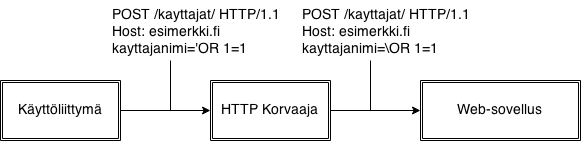
\includegraphics[scale=0.6]{http}
				\end{figure}
		
		\subsubsection{Parametrisoidut kyselyt}
		Parametrisoidut kyselyt esitellään artikkelissa "SQL injection vulnerability general patch using header sanitization"\space \cite{prepared}. Niiden avulla voidaan tallentaa käyttäjän antama syöte sellaisenaan tietokantaan, ilman että se muuttaa valmiiksi luodun kyselyn syntaksia. Tällöin "O'Brian" tallentuu "O'Brian":ina juuri kuten pitääkin. Parametrisoidussa kyselyssä luodaan SQL-kyselyistä pohjia, joihin lisätään paikanpitäjät (\textit{engl. placeholder}). Parametrisoitu kysely annetaan tietokannalle. Tietokanta kääntää ja optimoi kyselyn pohjan vain kerran. Tällainen toimintatapa parantaa suorituskykyä. Tietokanta ei kuitenkaan suorita varsinaista kyselyä heti, koska siitä puuttuu haettavat arvot. Kun käyttäjä antaa syötteenä haluamansa arvot, paikanpitäjät korvataan arvoilla. Käyttäjän antamia arvoja ei enää tulkata SQL:lläksi, vaan niitä käsitellään sellaisinaan. Tällöin ei ole mahdollista että käyttäjän syöte rikkoisi kyselyä. Esimerkiksi jos käyttäjä antaa käyttäjänimekseen "'; OR 1=1", niin tietokannasta haetaan käyttäjää, jonka käyttäjänimi on "OR 1=1".
		Parametrisoidut kyselyt ovat tuettuina lähes kaikissa yleisimmissä ohjelmointikielissä \cite{java}. Oikein käytettynä parametrisoidut kyselyt suojaavat sovelluksen täysin SQL-injektioilta \cite{prepared}.
		
		\subsection{Koodikatselmointi}
		Antunesin ja kumppaneiden tekemässä vertailussa\cite{vertailu} vertailtiin staattisen koodianalyysin ja penetraatiotestaamisen eroja. Kumpikaan testaustapa ei löytänyt yli 51\% sovelluksen tietoturva-aukoista. Tällaisten aukkojen huomaaminen on kuitenkin mahdollista, kun ohjelman lähdekoodia katselmoi useammat henkilöt.
		
		\subsection{Hienojakoinen pääsynhallinta tietokantaan}
		Tämä kappale keskittyy Roichmanin ja Gudesin artikkeliin "Fine-grained Access Control to Web Databases" \cite{access}.\space Artikkelin mukaan ennen web-sovellusten yleistymistä sovelluksia ajettiin käyttäjän omalla tietokoneella. Tyypillisellä sovelluksella oli kiinteä määrä  käyttäjiä. Tällaisessa sovelluskessa sovelluskerros kommunikoi suoraa tietokannan kanssa. Tämän seurauksena tietokanta tietää mikä käyttäjä sitä milloinkin käyttää. Täten on helppoa rajata käyttäjien oikeuksia.
						 \begin{figure}[h]
						 	\centering
						 	\caption{Web-sovelluksen kolme kerrosta.}
						 	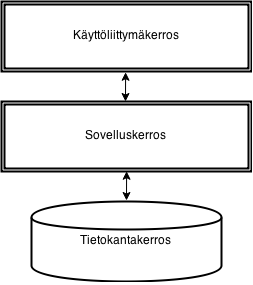
\includegraphics[scale=0.55]{kandi2}
						 \end{figure}
				 
				 
		 Nykyään web-sovelluksissa on tyypillisesti kolme kerrosta \cite{access}\cite{3tier}. Käyttöliittymänä toimii käyttäjän selain, joka kommunikoi web-sovelluksen palvelimen kanssa. Palvelin välittää käyttäjän käskyt tietokannalle. Tietokannan näkökulmasta komennot antaa web-sovellus, eikä komennon käyttöliittymästä lähettänyt käyttäjä. Täten tietokanta suorittaa sokeasti kaikki saamansa komennot, ellei web-sovellukseen tietokantakäyttäjän oikeuksia ole erikseen rajattu.
		

		 
		
		Aiemmin esitellyissä menetelmissä on keskitytty ratkaisemaan ongelmaa sovelluskerroksella. Roichmanin ja Gudesin lähestymistavassa keskitytään ratkaisemaan ongelmaa tietokantatasolla parametrisointi metodin \textit{(engl. parameter method)}) avulla. Tekniikka perustuu parametrisoituihin näkymiin \textit{(engl. parametrized views)}. Parametrisoidun näkymän avulla voi suodattaa tallenteita ilman, että tarvitsee tehdä uutta näkymään jokaista eri parametria varten.
		
		Sovelluksen tulee ylläpitää tietokantataulua johon merkataan aktiivisten käyttäjien ID:t. Roichamin ja Gudesin esittelemä metodi toimii seuraavalla tavalla:
		\begin{enumerate}
			\item Käyttäjä kirjautuu sovellukseen ja sovellus palauttaa käyttäjälle satunnaisen AS\_KEY:n, mikäli kirjautuminen onnistuu.
			
			\item Sovellus tallettaa aktiivisten käyttäjien tauluun käyttäjän ID:n ja sitä vastaavan AS\_KEY:n. Tästä lähin kaikissa käyttäjän tekemissä SQL-kyselyissä käytetään käyttäjäkohtaista AS\_KEY:tä.
			
			\item AS\_KEY poistetaan kun käyttäjä kirjautuu ulos.
		\end{enumerate}
		
		Kirjautumisen jälkeen käyttäjän tiedot ovat taulussa esimerkiksi seuraavalla tavalla:
	
		\begin{center}
		\begin{tabular}{| l | l | l | l |}
			\hline
			KäyttäjäID & AS\_KEY \\ \hline
			\hline
			20 &  01010101.. \\
			\hline
		\end{tabular}
		\end{center}
	

		Nyt voidaan käyttää seuraavanlaista parametrisoitua näkymää:
		\begin{lstlisting}
		CREATE VIEW Palkka_View WITH pAS_KEY
		SELECT * FROM Palkka
		WHERE Kayttaja_ID IN
		(SELECT Kayttaja_ID
		FROM Kayttajat_Table
		WHERE Kayttajat_Table.AS_key=:pAS_KEY) 
		\end{lstlisting}
		Näkymä ottaa parametrina AS\_Key:n, jonka käyttäjä on saanut kirjautuessaan. Käyttäjän kyselyt tehdään näkymään "Palkka\_View"\space eikä tauluun "Palkka". Mikäli hyökkääjä yrittäisi tehdä SQL-injektion tautologian avulla, suoritettava kysely näyttäisi seuraavalta:
		\begin{lstlisting}
			SELECT Palkka
			FROM Palkka_View(01010101..) 
			WHERE Palkka_pvm  = '12/2015' OR 1=1
		\end{lstlisting}
		Hyökkääjä saisi vastauksena kaikki omat palkkatietonsa, mutta ei muiden käyttäjien, koska Palkka\_View saa parametriksi hyökkääjän oman AS\_KEY:n. Myöskään UNION injektio ei ole tässä tapauksessa mahdollinen, koska hyökkääjä ei tiedä muiden käyttäjien AS\_KEY:tä, joka tarvitaan Palkka\_Viewiin parametriksi.
	
	\section{Ajonaikainen SQL-injektoiden estäminen}
	SQL-Injektioida voidaan yrittää havaita ja estää ajonaikana. Tätä varten on luotu useita työkaluja, kuten SQLCheck, SQLProb ja Candid. \cite{preventions}. Ajonaikaiseen SQL-injektioiden estämiseen on kehitetty monenlaisia tapoja. Tässä kappaleessa perehdytään tarkemmin AMNESIA, SQL-IDS ja SQLrand menetelmiin.
	
	\subsection{AMNESIA}
	Tässä kappaleessa esitellään artikkelissa "Preventing SQL Injection Attacks Using AMNESIA"\space\cite{amnesia} esiteltyä AMNESIA tekniikkaa. AMNESIA:n avulla pystytään estämään SQL-injektioida ajonaikaisesti. Artikkelin mukaan AMNESIA ottaa syötteenään sovelluksen lähdekoodin ja palauttaa siitä version, joka on suojattu SQL-injektiolta.
	
	 AMNESIA:ssa on ideana etsiä sovelluksen lähdekoodista ne paikat, joissa SQL-kyselyitä suoritetaan. Jokaista SQL-kyselyn suorituspaikkaa kohden luodaan ääreellinen automaatti. Automaatti hyväksyy vain ne syötteet, joita se ei tunnista SQL-injektoiksi. Ajon aikana jokaista suoritettavaa SQL-kyselyä verrataan suorituspaikkaa vastaavaan äärelliseen automaattiin. Kysely suoritetaan vain, mikäli automaatti hyväksyy syöytteen. AMNESIA tekniikka koostuu neljästä osasta:

	\begin{enumerate}
		\item{Etsi suorituspaikat}
		
		Ensin ohjelman koodi skannataan. Skannauksessa etsitään koodista ne paikat, joissa tietokantakyselyjä suoritetaan. Näihin paikkoihin viitataan tässä tutkielmassa sanalla "suorituspaikka" \textit{(engl. hotspot)}. Esimerkiksi Javan tapauksessa etsitään koodista paikat joissa kutsutaan "java.sql.Statement.execute(String)" \space metodia.
		\item{SQL-kyselymallien rakentaminen}
		
		Seuraavaksi rakennetaan jokaiselle edellisessä kohdassa löydetylle suorituspaikalle oma mallinsa. Tämä onnistuu siten, että AMNESIA simuloi sovelluksen toimintaa Java String Analysis (JSA) kirjaston avulla. JSA Luo analyysin tuloksena epädetermistisen ääreellisen automaatin (NDFA), joka tunnistaa kaikki mahdolliset merkkijonot, jotka kysely voi saada arvokseen. Esimerkiksi allaoleva koodipätkä voi saada arvokseen joko: 
		"SELECT info FROM kayttajat WHERE kayttajanimi = $\beta$"\space tai "SELECT info FROM kayttajat WHERE kayttajanimi='vieras'". Käyttäjän syötettä merkataan symbolilla $\beta$.
		
		\begin{lstlisting}
		query = "SELECT info FROM kayttajat WHERE"
		if (!kayttajanimi.empty) {
		query += "kayttajanimi ='" + kayttajanimi + "'"
		} else {
		query += "kayttajanimi = vieras"
		}
		\end{lstlisting}
		
		
		\item{Instrument application}
		
		Seuraavaksi lisätään jokaiseen vaiheessa 1. löydettyyn suorituspaikkaan monitori. Monitori suoritetaan aina ennen itse tietokantakyselyä. Monitori ottaa parametriksi suorituspaikan uniikin ID:n ja merkkijonon jota ollaan suorittamassa. ID:n avulla monitori etsii kyseistä suorituspaikkaa vastaavan mallin. Alla sama koodi esimerkkinä: 
		\begin{lstlisting}
		if (monitor.hyvaksyy(<suortuspaikan id>, kysely)) {
		return db.suorita(kysely);
		}
		\end{lstlisting}
		\item{Ajonaikainen monitorointi}
		
		Ajonaikana ohjelma toimii normalisti kunnes se törmää suorituspaikkaan. Suorituspaikkaan törmättyään se antaa tarvittavat parametrit monitorille. Ensin monitori käsittelee kyselyn samalla tapaa kuin tietokanta sen käsittelisi. Tämän asiosta esimerkiksi erikoismerkit evaluoituvat niiden oikeaan arvoonsa. Tämä estää SQL-avainsanojen piilottamisen erikoismerkeillä. Kun kysely on käsitelty, tarkastetaan tunnistaako malli sen. Mikäli malli hyväksyy kyselyn se suoritetaan, muulloin malli tunnistaa sen SQL-injektioksi.
		
		Oletetaan että kyselymme olisi "SELECT info FROM users WHERE kayttajanimi='' OR 1=1. Vaiheessa 1. kuvatun koodipätkän automaatti jakautuisi kahtia. Koska automaatti tunnistaa vain sellaiset kielet, jotka loppuvat merkkiin "\space'\space"\space heti käyttäjän syötteen jälkeen, kyseinen kysely huomataan SQL-injektioksi.
			\end{enumerate}
		\begin{figure}[h!]
		\caption{Vaiheen 2. koodia vastaava automaatti}
		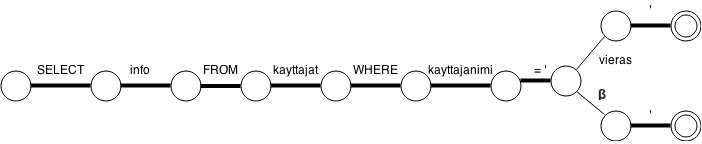
\includegraphics[scale=0.5]{kandi}
		\end{figure}

		\begin{figure}[b!]
			\caption{SQL-IDS lisättynä web-sovellukseen. SQL-IDS menetelmään liittyvät moduulit merkittynä vihreällä. \cite{sqlids}}
			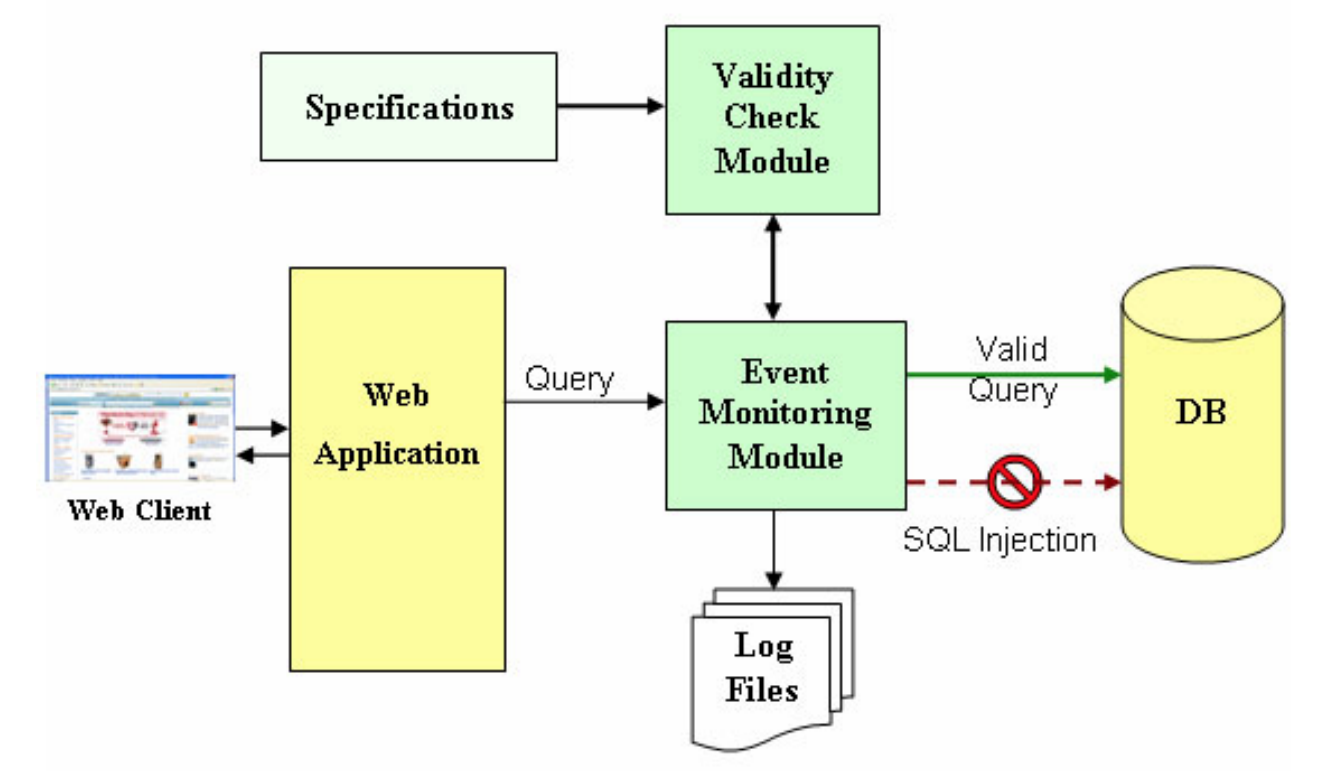
\includegraphics[scale=0.55]{sqlids}
		\end{figure}
		
	\subsection{SQL-IDS}
	SQL-IDS (SQL-Injection Detection System) esitellään Kemaliksen ja Theodroksen artikkelissa "SQL-IDS: A Specification-based Approach for SQL-Injection Detection"\space\cite{sqlids}. Se muistuttaa toimintatavaltaan AMNESIA:a, mutta siinä on joitakin eroavaisuuksia. AMNESIA vaatii muutoksia ohjelman lähdekoodiin, kun taas SQL-IDS on erillinen moduuli, joka asetetaan tietokannan ja sovelluksen väliin. AMNESIA Käyttää SQL-injektion tunnistamiseen äärellisiä automaatteja, kun taas SQL-IDS käyttää EBNF kielioppia.
	
	Artikkelin mukaan SQL-IDS menetelmässä sovelluksen ja tietokannan väliin asetetaan erillinen tapahtumaseurantamoduuli (\textit{engl. Event Monitoring Module}). Seurantamoduuli käsittelee sovelluksen lähettämiä SQL-kyselyitä antamalla ne oikeellisuuden tarkastusmoduulille (\textit{engl. Validity Check Module}). Mikäli tarkastusmoduuli hyväksyy SQL-kyselyn, se lähetetään tietokannalle. Muulloin kysely havaitaan SQL-injektioksi eikä sitä suoriteta. SQL-Injektioiksi havaituista kyselyistä kirjataan tietoja lokiin.
	
	Oikeellisuuden tarkastusmoduuli vastaanottaa SQL-kyselyn merkkijonona. Moduuli tulkkaa merkkijonon SQL:läksi, jonka jälkeen sitä verrataan ennaltamäärättyyn spesifikaatioon. Spesifikaatiot ovat määriteltyinä EBNF kieliopilla. Mikäli annettu lause ei riko kyseisen lauseen spesifikaatiossa määriteltyjä syntaktisia sääntöjä, se hyväksytään, jolloin se etenee seurantamoduulin kautta tietokannalle suoritettavaksi.

	Kemalis ja Theodoros ovat testanneet SQL-IDS menetelmää lähettämällä esimerkkisovellukselle 2450 SQL-kyselyä, joista 420 oli haitallisia. SQL-IDS onnistui tunnistamaan kaikki hyökkäykset. Artikkelin mukaan menetelmä lisää keskimäärin 1ms viiveen per SQL-kysely.
					

		
	\subsection{SQLRand}
	Boyd ja Keromytis esittelevät SQLRand menetelmän SQL-injektioiden torjumiseksi artikkelissaan "SQLRand: Preventing SQL Injection Attacks"\space \cite{sqlrand}. SQLRandissa on ideana lisätä jokaiseen SQL-avainsanaan jokin satunnainen numero.Alkuperäinen kysely voi näyttää esimerkiksi seuraavalta:

		\begin{lstlisting}[language=sql]
		SELECT * 
		FROM Oppilaat
		WHERE opintopisteet > 180
		\end{lstlisting}
		Kun SQLRand avaimena käytetään numeroa 123, valmis kysely näyttää seuraavalta: 
		\begin{lstlisting}[language=sql]
		SELECT123
		FROM123 Oppilaat
		WHERE123 opintopisteet > 180
		\end{lstlisting}
		
	
	
	Mikäli hyökkääjä yrittäisi suorittaa SQL-injektion tavallisilla SQL-avainsanoilla, se epäonnistuisi, koska sovellus ei tunnistaisi sitä SQL:läksi.
	
	Tavallinen tietokanta ei ymmärrä satunnaistettuja SQL-avainsanoja. Artikkelissa tähän ongelmaan oli luotu kaksi eri ratkaisua. Ensimmäinen on muokata tietokannan SQL-tulkkia siten, että se ymmärtää muokattuja SQL-avainsanoja. Tämä voi kuitenkin olla vaikeaa toteuttaa, sekä se saattaa sotkea muiden sovellusten toimintaa, jotka käyttävät samaa tietokantapalvelinta. Toinen ratkaisu on luoda erillinen tulkkisovellus tietokantapalvelimen ja web-sovelluksen välille.
	
	Boyd ja Keromytis esittelevät artikkelissaan myös SQLRandin tehokkuutta. Heidän mittaamiensa tulosten mukaan SQLRandin lisääminen tuo keskimäärin 183-316 mikrosekunnin viiveen per kysely.
	
	SQLRandia on kritisoitu sen monimutkaisuudesta \cite{prepared}. Kritisoijat pitävät SQLRandin toteuttamista olemassa olevaan sovellukseen aikaavievänä. Sen katsotaan myös hankaloittavan sovelluksen käyttöönottoa.
	\section{Penetraatiotestaus}
	
	 Vaikka sovellusta ohjelmoitaisiin hyvien ohjelmointikäytänteiden mukaisesti, siihen voi silti jäädä tietoturva-aukkoja. Tämän takia sovellusta on jatkuvasti tietoturvatestattava. 
	 
	 Penetraatiotestauksessa yritetään etsiä sovelluksesta tietoturva-aukkoja. Kun penetraatiotestaus on automatisoitua, ohjelmoijan ei tarvitse suorittaa samoja testausruutineja käsin jokaisen muutoksen jälkeen. Penetraatiotestaus ei kuitenkaan ole virheetöntä. Artikkelissa "Using web security scanners to detect vulnerabilities in web services" \cite{detection} kerrotaan, että penetraatiotestaus voi aiheuttaa turhia hälyytyksiä, tai olla hälyyttämättä kun pitäisi hälyyttää. Artikkelin mukaan jopa yli 30\% havaituista virheistä osoittautuivat virheellisiksi. Tämän takia penetraatiotestauksen tulee olla vain yksi testaustyökaluista, eikä siihen voida sokeasti luottaa.
	 
	Musta laatikko -testauksessa testataan sovellusta erilaisia syötteitä vastaan. Tällaiseen testaamiseen ei vaadita pääsyä itse koodiin \cite{testing2}. Tämä on hyödyllistä esimerkiksi sellaisissa tapauksissa, kun osa ohjelman komponenteista on kolmannen osapuolen koodia, eikä siihen päästä käsiksi. Mustalaatikko testauksessa on ongelmana se, että tulos perustuu sovelluksen tulosteesta tehtyyn analyysiin, eikä esimerkiksi tietokannan todelliseen tilaan. Tästä syystä kaikkia tietoturva-aukkoja ei välttämättä löydetä, tai jotain turvallista kohtaa koodista voidaan luulla tietoturva-aukoksi. Mustalaatikkotestaukseen löytyy useita valmiita työkaluja, kuten "Acunetix Web Vulnerability Scanner"\space ja sqlmap.
	
	Valkolaatikko testauksessa testaajalla on pääsy ohjelman lähdekoodiin. Valkolaatikko testaustyökaluihin kuuluu esimerkiksi staattiset lähdekoodin analysointi työkalut. Tällaisilla työkaluilla voidaan huomata mahdollisia tietoturva-aukkoja jo ennen kun ohjelmaa on ajettu ensimmäistäkään kertaa \cite{valkolaatikko}.
	
	Tässä kappaleessa esitellään ehdotettu malli siitä, kuinka penetraatiotestaus työkalut kannattaa toteuttaa, kuinka testaussyötteidä voidaan luoda automatisoidusti, sekä kuinka V1p3R penetraatiotestaustyökalu toimii.
	
	\subsection{Penetraatiotestauksen toiminta}
	 Haixia edottaa artikkelissaan "A database security testing scheme of web application"\space\cite{testing} seuraavanlaista testausmallia.
	
	Ensiksi etsitään kaikki mahdolliset paikat sovelluksesta, joista käyttäjä voi syöttää dataa. Tämä onnistuu leveyssuuntaista hakua (\textit{engl. Breadth-first search}) käyttämällä. Algoritmi toimii seuraavasti:
	\begin{enumerate}
		\item Alustetaan lista jossa on ainoana jäsenenä etusivun URL. Etusivu merkataan käsittelemättökäks.
		
		\item Käydään listalta läpi kaikki käsittelemättömiksi merkatut sivut. Kunkin sivun kohdalla tehdään seuraavat vaiheet:
		
		- Otetaan talteen kaikki paikat joista käyttäjä voi syöttää dataa.
		
		- Etsitään sivulta kaikki linkit ja lisätään listalle ne jotka eivät vielä ole siellä.
		
		- Merkataan sivu käsitellyksi.
		
		\item Mikäli listalla on käsittelemättömiä linkkejä, palataan vaiheeseen 2.
	\end{enumerate}
	
	Tämän jälkeen luodaan mahdollisimman kattava lista erilaisista hyökkäyksistä. Listan luomiseen esitellään menetelmä seuraavassa kappaleessa. Kaikkiin mahdollisiin paikkoihin joista voi syöttää dataa kokeillaan haitallisia syötteitä. Tietokannan palauttamasta arvosta voidaan päätellä onko injektio onnistunut vai ei. Esimerkiksi jos vastauksen HTTP statuskoodi on 200, kyseessä on haavoittuvuus. 
	
	\subsection{Testaussyötteiden luominen}
	Artikkelissa "Automated Testing for SQL Injection Vulnerabilities: An input Mutation Approach"\cite{generation}\space ehdotetaan penetraatiotestauksessa käytettävien syötteiden luomiseen automatisoitua tekniikkaa nimeltään $\mu$SQLi. Tekniikassa on ideana manipuloida kelpaavaa syötettä erilaisilla mutaatio-operaatioilla. Mutaatio-operaatiot jaetaan artikkelin mukaan seuraavalla tavalla kolmeen eri osioon:
	\begin{enumerate}
	\item Käyttäytymistä muuttavat operaatiot
	
	Esimerkiksi operaatiot jotka lisäävät AND tai OR lauseen, tai operaatiot joissa lisätään puolipiste ja kokonaan uusi SQL lause. 
	
	\item Syntax-Repairing Operators
	
	Lisää kyselyyn esimerkiksi sulut, kommenttimerkin tai heittomerkin.
	
	\item Obfuskointi operaatiot
	
	Esimerkiksi muuttaa kyselyssä käytettävää enkoodausta tai muuttaa totuuslauseketta ilman että sen arvo muuttuu.
	\end{enumerate}
	
	Toimivaan syötteeseen voidaa lisätä yksi tai useampi mutaatio-operaatio. Artikkelin mukaan useasti yksittäinen operaatio huomataan, mutta yhdistelmät saattavat silti jäädä huomaamatta. Mutaatioiden tekeminen aloitetaan toimivasta syötteestä, koska sillä vältetään se, että syöte hylättäisiin välittömästi. Lisäksi toimivat syötteet täyttävät todennäköisemmin syötevalidoinnit. 
	
	\subsection{V1p3R}
	V1p3R on Visaggion ja Di Pentan kehittämä penetraatiotestaus työkalu. Se on esitelty artikkelissa "A Heuristic-based Approach for Detecting SQL-injection Vulnerabilities in Web Applications"\space\cite{viper}. Artikelissa esiteltyjen testitulosten mukaan V1p3R on tehokkaampi kuin tunnetu sqlmap työkalu. Se tunnistaa enemmän SQL-injektioon liittyviä tietoturva-aukkoja pienemmällä määrällä kokeiluja. Vertailu tehtiin kahdellatoista oikeasti käytössä olevalla web-sovelluksella.
	
	Artikkelin mukaan suurin osa penetraatiotestaus työkaluista toimii edellisten kappaleiden kuvaamalla tavalla: etsitään sovelluksesta injektoitavat URL:it ja lomakkeet, jonka jälkeen suoritetaan niihin satunnaisia SQL-injektioita. Myös V1p3R aloittaa testaamisen lähettämällä satunnaisia kyselyitä, mutta testaaminen ei lopu siihen. Hyökkäysten edetessä V1p3R oppii lisää kohteena olevasta sovelluksesta ja muodostaa hyökkäykset oppimansa perusteella.
	
	 Viper osaa kerätä tietokannasta tietoja huolimatta siitä vastaako sovellus virhesivulla, vai toimivalla näkymällä. Mikäli sovellus vastaa virhesivulla, V1p3R vertaa virheilmoitusta säännöllisiin lausekkeisiin (\textit{engl. regular expression}). Viper voi päättellä säännöllisten lausekkeiden avulla virheilmoituksesta seuraavia asioita:
	 \begin{itemize}
	 	\item Tietokannan hallinnointijärjestelmä (DBMS)
	    \item Suoritettavan kyselyn rakenne
		\item Tietokantataulujen ja kenttien nimiä
	\end{itemize}
	
	Mikäli SQL-injektio ei aiheuta virhesivua, V1p3R pystyy myös silloin päättelemään asioita tietokannan rakenteesta. Artikkelissa annetaan seuraavanlainen esimerkki: Mikäli injektoitava URL on: \textit{http://www.dotcom.com/itemID.jsp?itemID=6} ja itemID muutetaan \textit{6 AND 1=1}, haavoittuvainen sovellus palauttaa saman tuloksen, kuin pelkkä 6 palauttaisi. Sen sijaan suojattu sovellus palauttaa todennäköisesti eri tuloksen. Asettamalla 1=1 tilalle muita propositiolauseita V1p3R pystyy päättelemään lisää tietokannan rakenteesta. Esimerkiksi \textit{ASCII(SUBSTRING(username,1,1))=97 } lauseella voidaan päätellä onko username taulun ensimmäinen kirjain a, jatkamalla tätä voidaan päätellä username taulun kaikkien kenttien nimet.
	
	Kun V1p3R on kerännyt sovelluksesta kaikki mahdoliset tiedot, se raportoi tulokset lokitiedostoihin. Lokitiedostot sisältävät tiedot haavoittuvista URL:leista, lomakkeista sekä HTTP-headereista. Näiden tietojen avulla ohjelmoija voi todentaa tietoturva-aukkojen olemassa olon ja korjata ne.
	
	
	\section {Yhteenveto}
	SQL-Injektiot ovat olleet web-sovelluksien uhkana jo kauan. Niiltä suojautumiseen on kehitetty monenlaisia toimivia suojautumismenetelmiä. Osa menetelmistä suojaa sovelluksen täydellisesti, mutta osa vain hankaloittaa hyökkäystä. Esimerkiksi parametrisoidut kyselyt suojaavat sovelluksen SQL-injektoilta täydellisesti, kunhan niitä käytetään oikein. Sen sijaan esimerkiksi syötteen validointi ei takaa suojaa SQL-injektioilta, mutta saattaa hankaloittaa hyökkäystä.
	
	Osa suojautumismenetelmistä täytyy olla mukana ohjelmointityylissä alusta loppuun asti, sillä niiden lisääminen myöhemmin on työlästä. Esimerkiksi parametrisoidut kyselyt tai Roichmanin ja Gudesin esittelemä hienojakoinen pääsynhallinta tietokantaan vaikuttavat moneen paikkaan lähdekoodissa. Osa tekniikoista sen sijaan voidaan ottaa käyttöön vaivattomasti myöhämmässäkin vaiheessa. Esimerkiksi Sadeghanin ja Zamanin esittelemä HTTP-pakettienkäsittelijä, joka voidaan asettaa käsittelemään HTTP-paketteja ennen kun ne annetaan sovellukselle, on helppoa lisätä olemassa olevaan sovellukseen. 
	
	Suojautumismenetelmiä on kehitetty eri tasoille web-sovellusta. Esimerkiksi edellämainittu HTTP-pakettienkäsittelijä asetetaan käsittelemään paketit ennen kuin ne annetaan sovellukselle. Parametrisoiduilla kyselyillä ja validoinnilla pyritään estämään SQL-injektoita sovelluksen lähdekoodissa. SQL-IDS Menetelmässä sen sijaan injektioilta pyritään suojautumaan ennen kuin kysely suoritetaan kannassa. Hienojakoisessa pääsynhallinnassa sen sijaan injektioilta suojautuminen toteutetaan vasta tietokantatasolla.
	
	Jotkin menetelmistä heikentävät suorituskykyä tai vaikeuttavat ohjelman käyttöönottoa. Esimerkiksi AMNESIA tekniikkaa käyttäessä sovellus täytyy jokaisen muutoksen jälkeen käsitellä AMNESIA työkalulla. Toisaalta AMNESIA työkalua käyttäessä SQL-injektioilta suojautumiseen ei tarvitse juurikaan käyttää aikaa ohjelmoinnin aikana, sillä AMNESIA hoitaa suojautumisen automatisoidusti.
	
	Jotta suojautumisen onnistumisesta voitaisiin varmistua, sovellusta on testattava. Sovelluksen testaamiseen on luotu erilaisia valmiita työkaluja. Osa työkaluista, kuten staattiset koodin analysointityökalut vaativat pääsyn ohjelman lähdekoodiin. Osa toimii pelkästään ohjelman antaman palautteen perusteella. Tämän hetkisiä työkaluja yhdistää korkeat "false-positive"\space prosentit. Tästä syystä testaustyökalujen antamista tuloksista ei voida päätellä varmaksi, onko sovellus turvallinen vai ei. Koska teustaustyökalujen antamien tulosten oikeellisuudesta ei voida olla varmoja, ohjelmoijan on myös itse ymmärrettävä mikä on SQL-injektio.
	
	 Erilaisia suojautumismenetelmiä on niin laaja kirjo, että jää epäselväksi milloin mitäkin suojautumismenetelmää kannattaa käyttää. Tutkielmaa voisi jatkaa tutkimalla tätä asiaa.
	
	



	% --- References ---
	%
	% bibtex is used to generate the bibliography. The babplain style
	% will generate numeric references (e.g. [1]) appropriate for theoretical
	% computer science. If you need alphanumeric references (e.g [Tur90]), use
	%
	% \bibliographystyle{babalpha-lf}
	%
	% instead.
	
	\bibliographystyle{babalpha-lf}
	
	\bibliography{references-fi}
	
	
	% --- Appendices ---
	
	% uncomment the following
	
	% \newpage
	% \appendix
	% 
	% \section{Esimerkkiliite}
	
\end{document}